
\section{Multivariate analysis}
\label{sec:mva}

After the traditional cut-based analysis presented in the previous section,
and combining the significance of the different event categories,
we end up with a $S/\sqrt{B}$ value of AAA.
%
Taking into account our more realistic simulation of the QCD background as
compared to previous studies, this is not too bad.
%
However, the attentive reader might have noticed that we have used
relatively 
loose kinematics cuts, for example in the Higgs mass window.
%
The motivation for this is that the $n$-tuples of signal and background
events, after our basic selection, are processed though a multivariate
analysis with the motivation to increase the signal over background
significance.
%
Multivariate techniques are by now a common tool to enhance signal
significance in HEP analysis.

\subsection{MVA strategy}

The final step of our analysis is to process our three exclusive
categories of events (boosted, intermediate and resolved) though
a Multivariate Analysis.
%
The particular tool that we adopt is
a feed-forward artificial neural network.\footnote{This is the
  same type of neural networks as those used in the
  NNPDF analysis of parton distributions~\cite{Ball:2010de}.}
%
The architecture of the neural network is
\be
\label{eq:nn1}
N_{\mathrm{var}}\times5\times3\times1 \, ,
\ee
with $N_{\mathrm{par}}$ the number of input variables for the MVA.
%
Therefore, we have two hidden layers and a single output variable, which
is the value of the discriminant to separate signal and background.\footnote{Note that in the MVA literature artificial neural networks with several hidden
  layers are known as {\it deep neural networks}.}
%
Below we list the variables that are given as input to the MVA in each
different category.
%
The MVA has trained using a Genetic Algorithm during 50K iterations,
and the figure of merit to be minimized is the cross-entropy function.
%
This figure of merit is defined as
\be
\bf DEF
\ee

For both signal and background events, the variables that we input
to the MVA are the following.
%
For the boosted category we have
\begin{itemize}
\item The invariant mass of the two mass-drop-tagged jets, $m_{\rm jet}$
\item The transverse momentum of the reconstructed Higgs pair, $p_{T,hh}$
\item The rapidity of the two mass-drop-tagged jets, $y_{\rm jet}$
\item The invariant mass of the leading Higgs candidate, $m_{h,1}$
\item The invariant mass of the sub-leading Higgs candidate, $m_{h,2}$
\item The splitting scale of the first Higgs
\item The splitting scale of the second Higgs
\item The subjetiness variable $\tau_{21,h1}$ of the leading Higgs candidate
\item The subjetiness variable $\tau_{21,h2}$
  of the sub-leading Higgs candidate
 \item The angular separation between the two tagged jets, $\Delta R_{1,2}$ 
\end{itemize}
For completeness, we give here the definition of the various substructure variables.
%
The splitting scale is defined as
\be
\bf DEF
\ee
while the $\tau_{1,2}$ subjetiness variable is defined as
\be
\bf DEF
\ee
The other variables are more conventional.
%
As will be shown below, the addition of the jet substructure variables,
the splitting scales and the subjetiness,
enhances substantially the signal significance, as compared
to using only jet variables without substructure information.

For the resolved analysis instead, the $N_{\rm var}$ kinematic variables
that are given as input to the MVA are the following
\begin{itemize}
\item The invariant mass of the four $b$-tagged leading jets (that
  is, of the di-Higgs system), $m_{4b}$
\item The transverse momentum of the di-Higgs system, $p_{4b}$
\item The rapidity of the di-Higgs system $y_{4b}$
\item The invariant mass of the leading Higgs candidate $m_{h,1}$
\item The invariant mass of the subleading Higgs candidate $m_{h,1}$
\item The angular separation between each of the four
  $b$-tagged leading jets in the event: $\Delta R_{b1,b2}$,
  $\Delta R_{b1,b3}$, $\Delta R_{b1,b4}$, $\Delta R_{b2,b3}$,
  $\Delta R_{b2,b4}$, $\Delta R_{b3,b4}$
\end{itemize}
As will be shown below, of all these variables, the invariant mass of the
Higgs candidates is the one that carries as higher discrimination
power.

\subsection{Enhancing signal discrimination with the MVA}

Now we show the results of the MVA training on the signal and
background samples.
%
First of all in Fig.~\ref{fig:nnresponse} we show
the neural network classification of events is demonstrated for both the resolved and boosted cases.
%
In this figure, we show which is the distribution of the neural network
response, that is, the value of the outer layer in Eq.~(\ref{eq:nn1}),
for signal and background events.
%
For the MVA discrimination to be successful, one needs to find
distinct distributions for the two types of events.
%
As can be seen from  Fig.~\ref{fig:nnresponse}, both
in the boosted and in the resolved cases signal and background
distributions are noticeably different: we can use this property
to introduce the final cut in our analysis, a cut in the value
of the neural network output.

%%%%%%%%%%%%%%%%%%%%%%%%%%%%
\begin{figure}[t]
\begin{center}
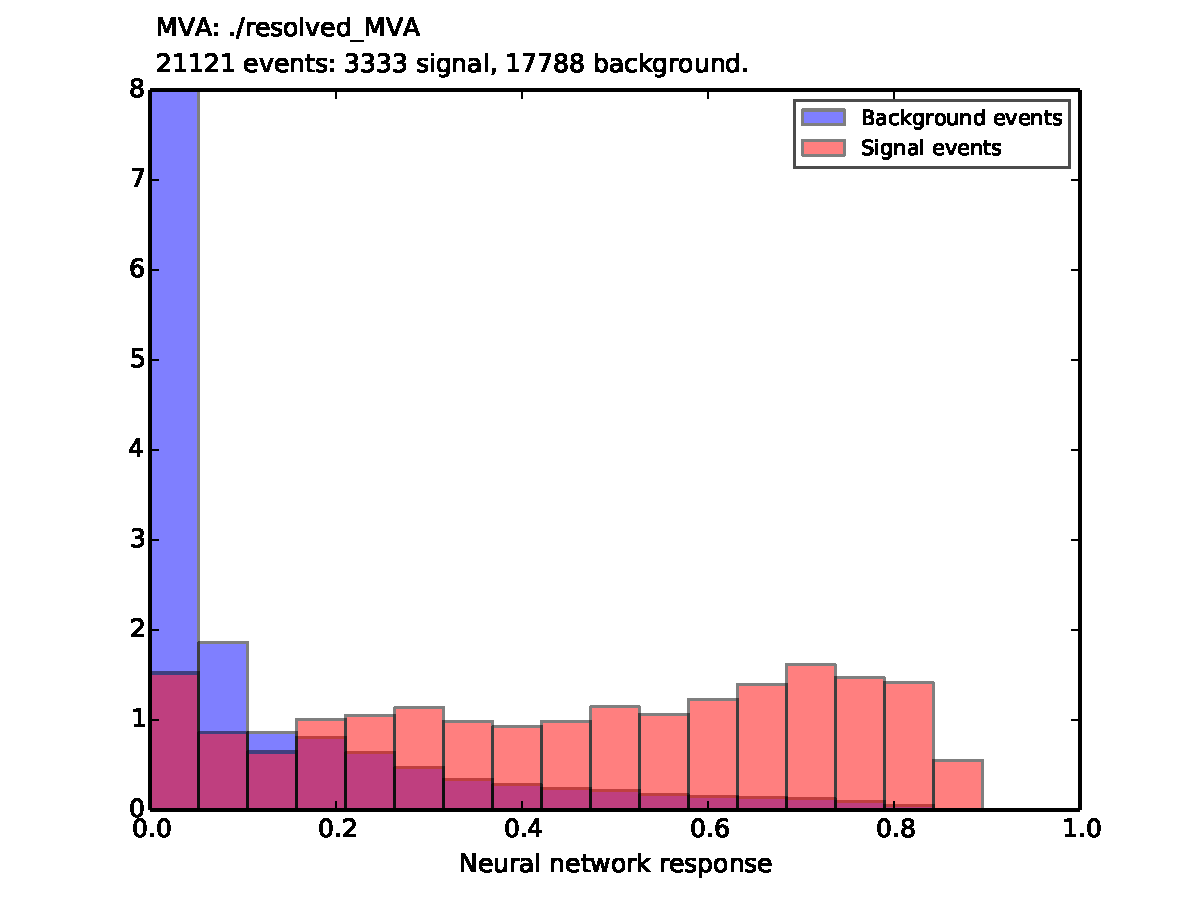
\includegraphics[width=0.48\textwidth]{plots/resolved_MVA_hist.pdf}
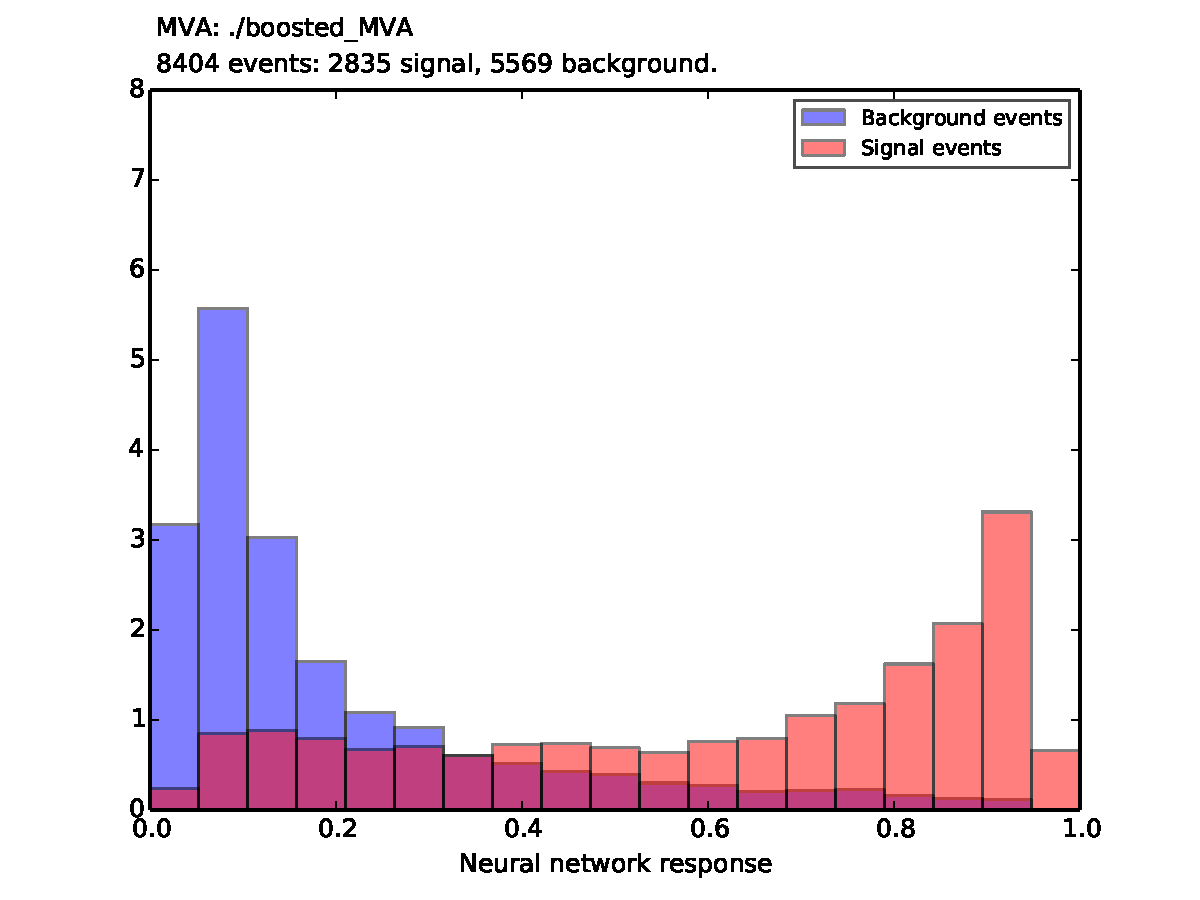
\includegraphics[width=0.48\textwidth]{plots/boosted_MVA_hist.pdf}
\caption{\small Neural network response demonstrated for the case of the resolved (left) and boosted (right) analyses. The frequency of background and signal events is plotted as a function of neural network output.
{\bf what is the y axis??}
}
\label{fig:nnresponse}
\end{center}
\end{figure}
%%%%%%%%%%%%%%%%%%%%%%%

The result of the signal selection efficiency as a function of the
background rejection rate as the value on the cut on the NN output
is varied is known as the Receiver Operating Characteristic (ROC)
curve.
%
It is clear that we can achieve a very high signal efficiency but using
a low value of the threshold, but this will have a poor background
rejection.
%
Using a higher value of the cut will increase background rejection at the
cost of dropping signal efficiency.
%
The usefulness of ROC curves is that they allow to determine the
optimal cut value that removes enough background without degrading too much the signal efficiency.

In Figure~\ref{fig:exampleroc} the ROC curves for the two analyses are shown, demonstrating that the neural network is able to
perform well in both cases. Figure~\ref{fig:nnweights} shows the distribution of NN weights in both cases.

%%%%%%%%%%%%%%%%%%%%%%%%%%%%%%%%%%%%%%%%%%%%%%
\begin{figure}[t]
\begin{center}
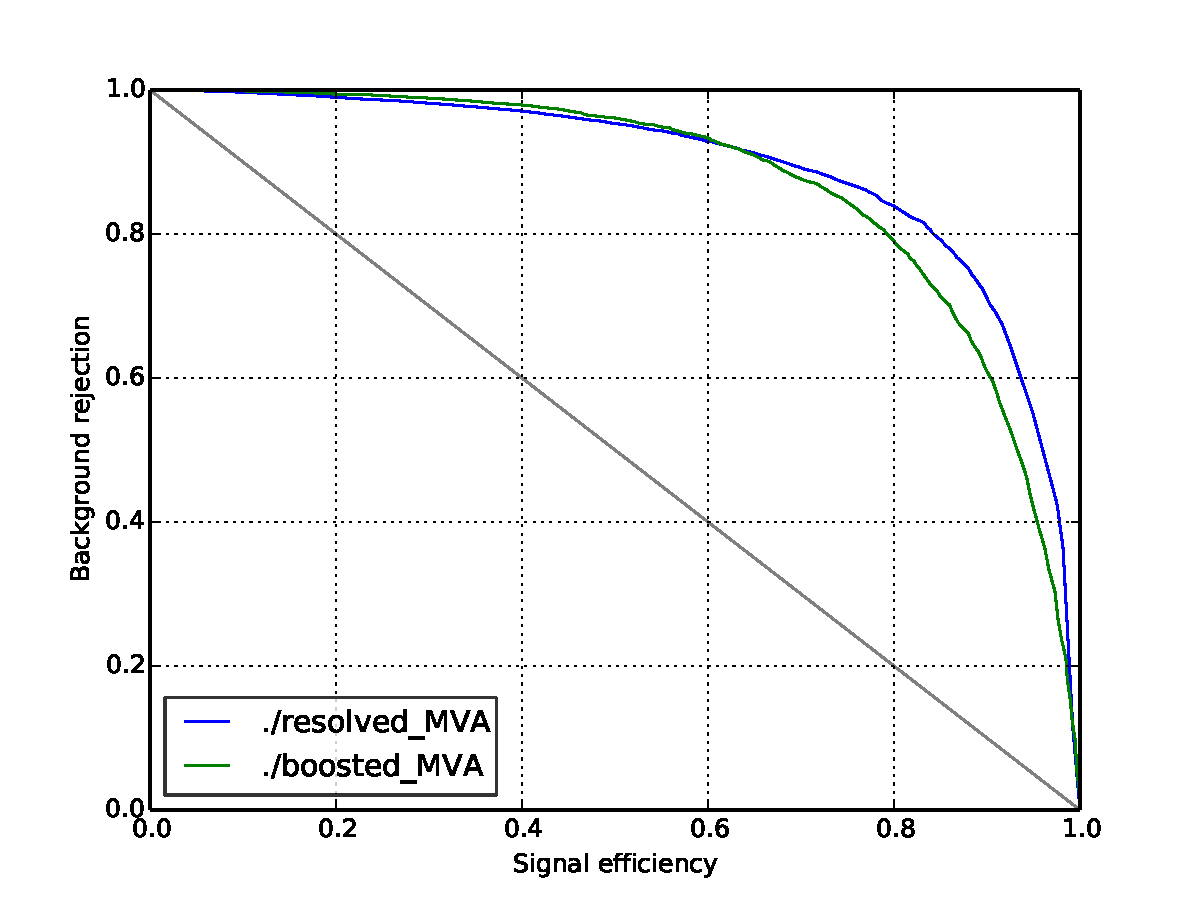
\includegraphics[width=0.65\textwidth]{plots/example_roc.pdf}
\caption{\small ROC curve for the neural network discriminant in the boosted (green) and resolved (blue) cases.}
\label{fig:exampleroc}
\end{center}
\end{figure}
%%%%%%%%%%%%%%%%%%%%%%%%%%%%%%%%%%%%%

\begin{figure}[h]
\begin{center}
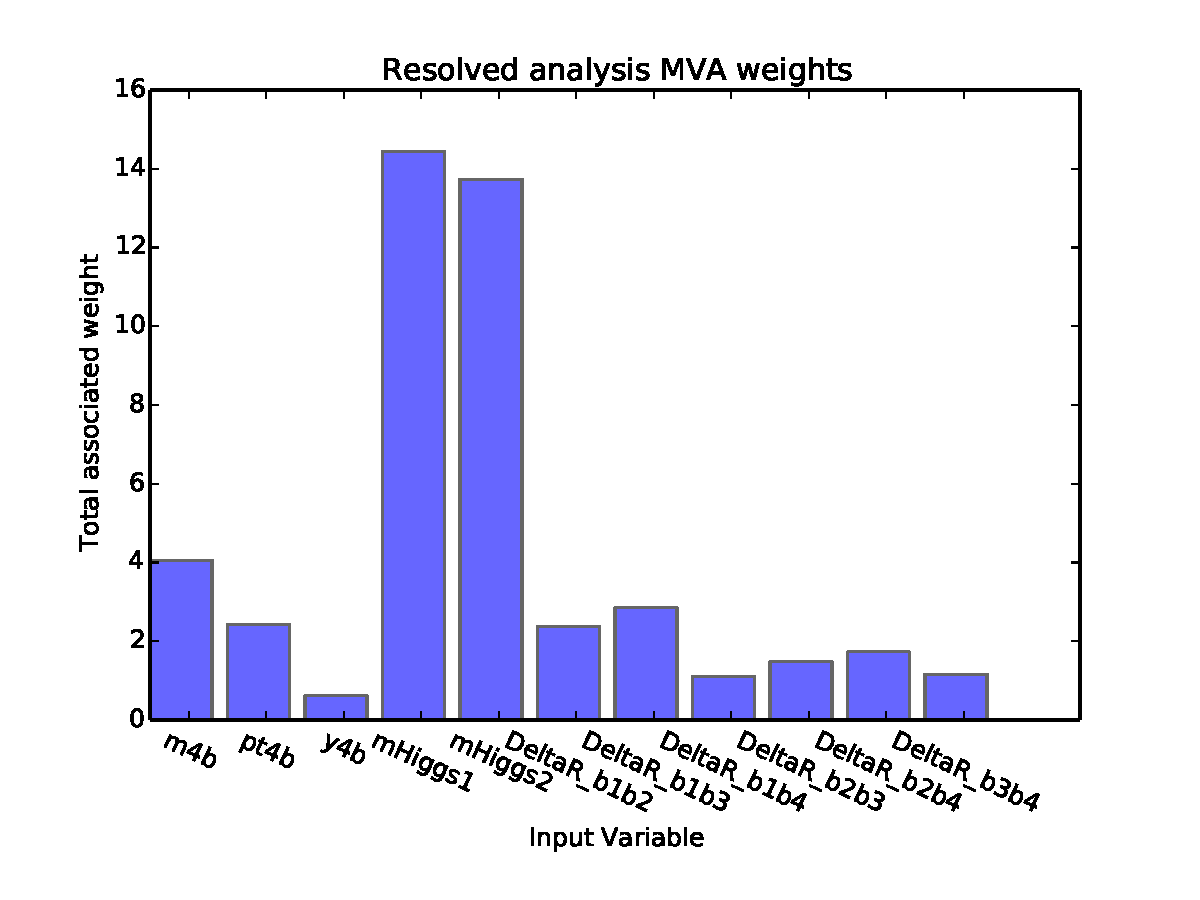
\includegraphics[width=1\textwidth]{plots/nnweights_res.pdf}
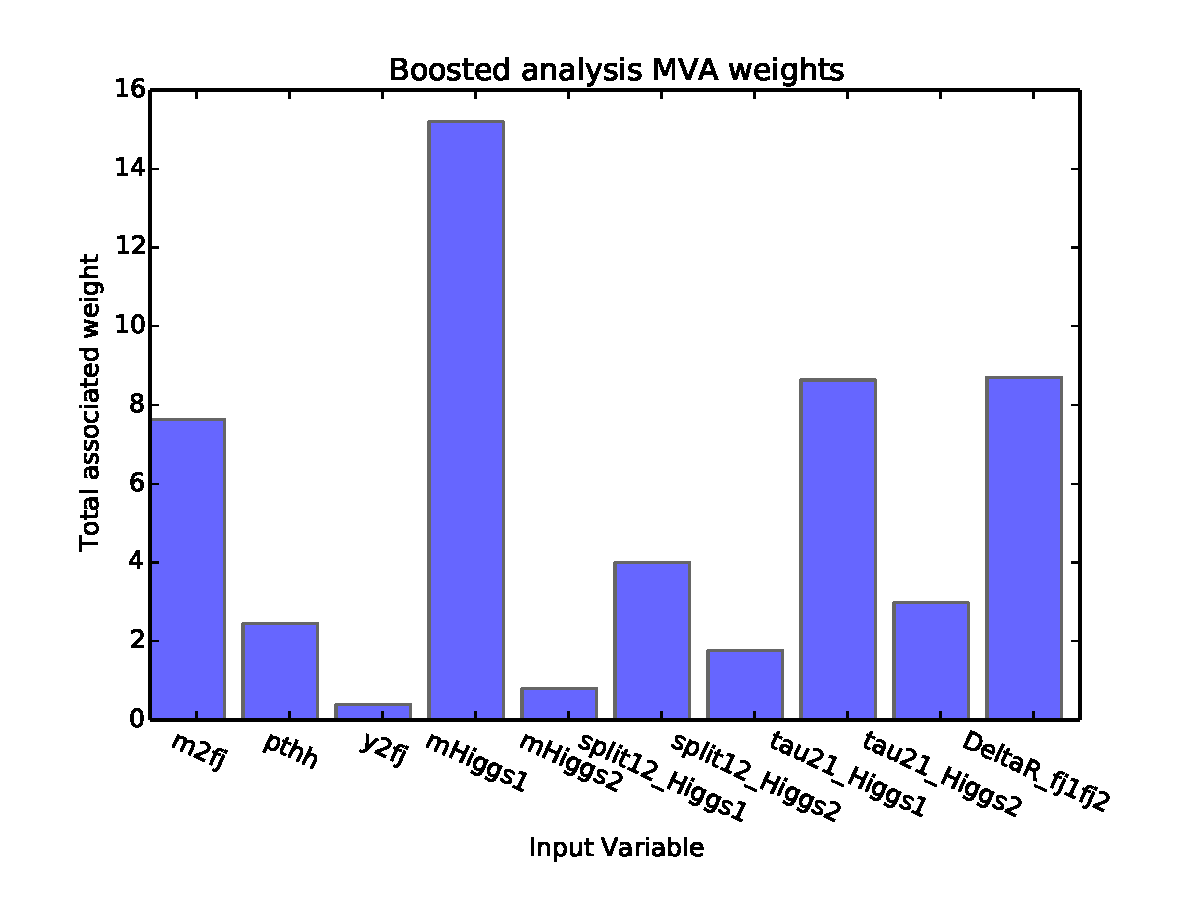
\includegraphics[width=1\textwidth]{plots/nnweights_boost.pdf}
\caption{Distribution of weights per input variable in the final ANN analysis. The above figure shows the weight distribution in the case of the resolved analysis, while the lower plot shows the boosted analysis.}
\label{fig:nnweights}
\end{center}
\end{figure}
\clearpage

Figure~\ref{fig:nnweights} demonstrates that the dijet invariant mass is a crucial variable for the resolved analysis MVA. As no detector effects were modeled in this analysis, it is reasonable to assume that the MVA has greater discriminating power than would be feasible in a real analysis. To investigate this, we now consider a variant of the analysis used in Table~\ref{tab:resCutflow} where the $m_H$ window criterion has been relaxed to $80 < m_H < 170$. Firstly the same analysis is repeated with the larger $m_H$ window. This is then compared to the same analysis but with a Gaussian smearing with $\sigma=10$ GeV applied to the dijet invariant mass used in the MVA. In the left panel of Figure~\ref{fig:invMsmear} the smearing is demonstrated. Despite the smearing, the MVA applied to this analysis still vastly prefers the dijet masses as discriminators, as is demonstrated in the right panel of Figure~\ref{fig:invMsmear}.
  

While the MVA still derives most of it's discriminating power from the dijet masses, the smearing reduces it's effectiveness considerably. In Figure \ref{fig:smearedROC} the ROC curves of the MVA applied to the smeared and unsmeared distributions are shown, where it is clear that the overall performance of the MVA is significantly hampered by the smeared invariant masses. This is echoed in the resulting significance of the analysis as demonstrated in Figure~\ref{fig:smearedSB}
